\documentclass{jarticle}
\usepackage[dvipdfmx]{graphicx}
\usepackage{here}
\usepackage{listings,jlisting}


\lstset{
  basicstyle={\ttfamily},
  identifierstyle={\small},
  commentstyle={\smallitshape},
  keywordstyle={\small\bfseries},
  ndkeywordstyle={\small},
  stringstyle={\small\ttfamily},
  frame={tb},
  breaklines=true,
  columns=[l]{fullflexible},
  numbers=left,
  xrightmargin=0zw,
  xleftmargin=3zw,
  numberstyle={\scriptsize},
  stepnumber=1,
  numbersep=1zw,
  lineskip=-0.5ex
}

\title{{システム実験}\\実験10回レポート}
\author{6119019056 山口力也}
\date{2019/06/28日提出}

\begin{document}
\maketitle
\section{I-P制御}
\subsection{目的}
課題6.1の目的は何か?90字以上で答えよ. \\

課題6.1では,モータの回転速度を目標値に一致させるI-P制御系の設計方法を取得することを目的とした.
$\sigma = 0.5$として,比例ゲイン$K_P$と積分ゲイン$K_I$を定め,目標値の矩形波の理論的な出力応答と,実際の応答で時定数とゲインが合っているかどうか確かめた.この時,モータ回転速度の原点をY0として比例フィードバックした.
\subsection{フィードバックゲイン}
フィードバックゲイン$K_P$,$K_I$および$(U_0,Y_0)$を報告せよ.ただし値を報告するだけだけでなく,どのように求めたか説明すること.


$\sigma= 0.5$として求めると
\begin{equation}
\frac{1 + 34000K_P}{34000K_I} = \sigma = 0.5
\end{equation}

\begin{equation}
\frac{0.5}{34000K_I} = 0.5\sigma^2 = 0.5 = 0.125
\end{equation}

より,
\begin{equation}
K_I = 0.00012 = 1.2 \times 10 ^{-4}
\end{equation}

\begin{equation}
K_P = 0.00003 = 3.0 \times 10 ^{-5}
\end{equation}

また,計測値から非線形システムから線形システムへの近似を考えて
\begin{equation}
U_0 = 0.2
\end{equation}

\begin{equation}
Y_0 = 1950.0
\end{equation}
とした.

\subsection{実験結果}
課題6.1-2の結果を報告せよ.その際,モータの回転速度,duty比,目標回転速度などのデータをScilabを用いてグラフにすること. \\

以下図\ref{fig:kadai6-1-1-1}にモータの回転速度と目標回転速度のグラフを示す.

\begin{figure}[H]
\begin{center}
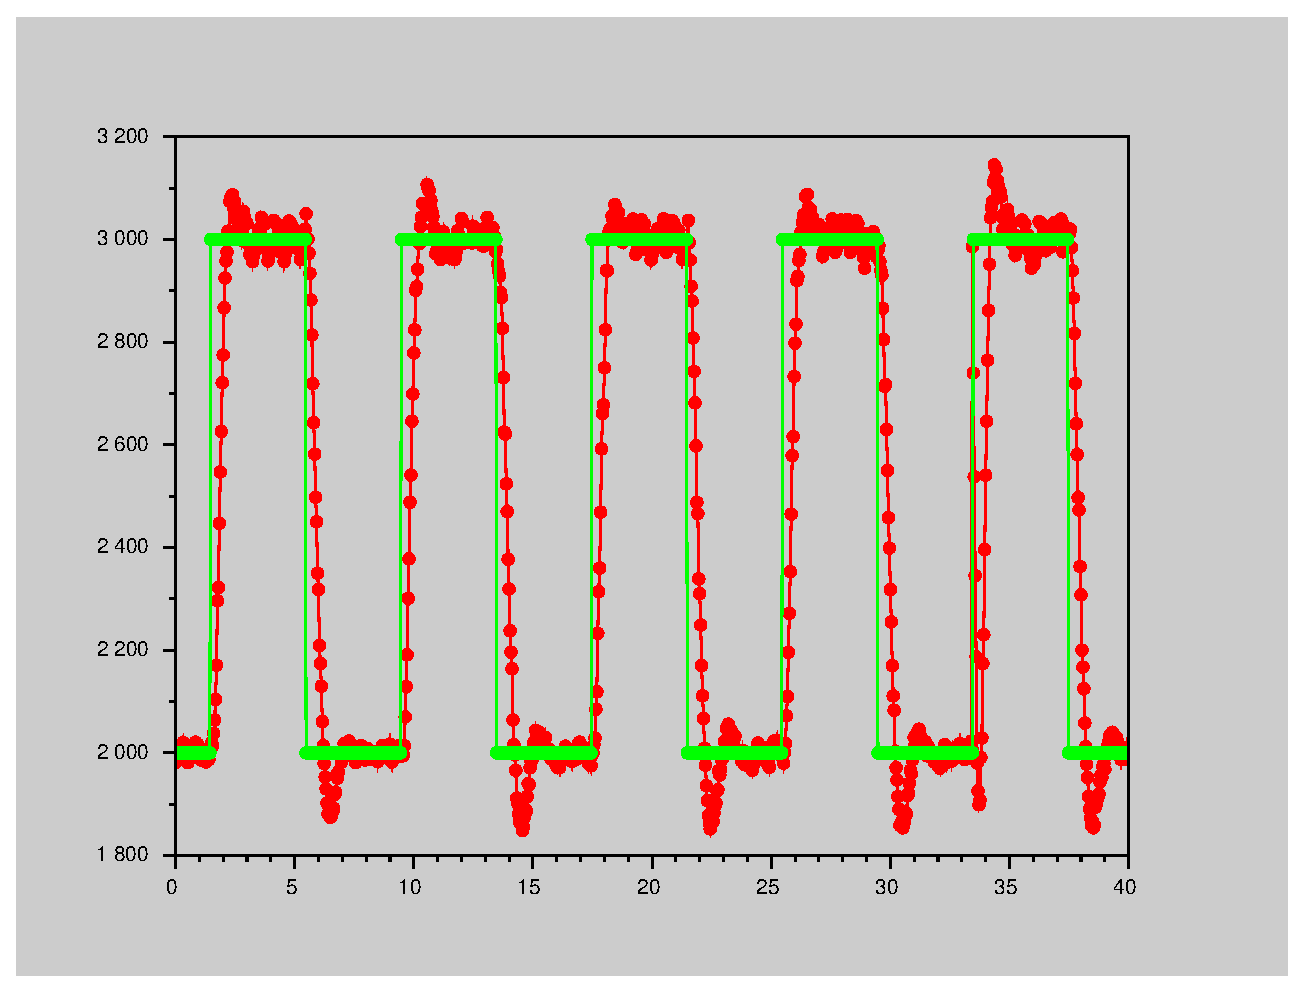
\includegraphics[width=7.0cm]{images/kadai6-1-1-1.eps}
\caption{モータの回転速度と目標回転速度のグラフ}
\label{fig:kadai6-1-1-1}
\end{center}
\end{figure}

以下図\ref{fig:kadai6-1-1-2}にduty比と時間のグラフを示す.

\begin{figure}[H]
\begin{center}
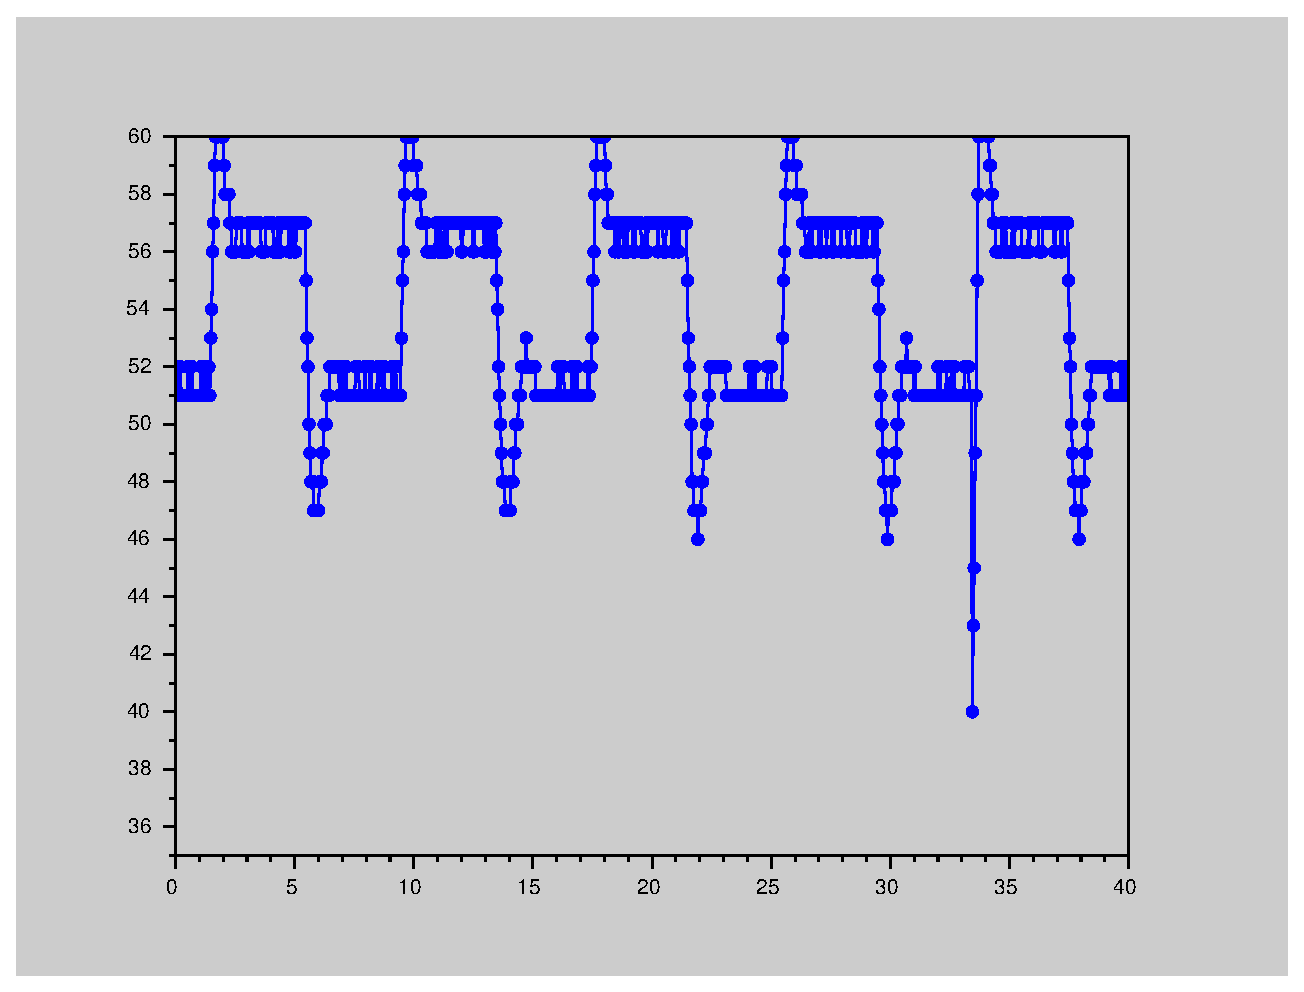
\includegraphics[width=7.0cm]{images/kadai6-1-1-2.eps}
\caption{duty比と時間のグラフ}
\label{fig:kadai6-1-1-2}
\end{center}
\end{figure}

\subsection{$K_P$の影響}
課題6.1-3の結果を報告せよ.$K_P$の値の違いによる応答の違いをグラフを用いて説明せよ.$K_P$の役割や調整の仕方について考察せよ.Scilabによるグラフの作成では,3つの応答の時間軸を調整して1つのグラフに描き,時定数などを比較できるようにせよ.

以下図\ref{fig:kadai6-1-3}に$K_I$の値を変えず$K_P$の値を1倍,2倍,0.5倍としたときのグラフを示す.

\begin{figure}[H]
\begin{center}
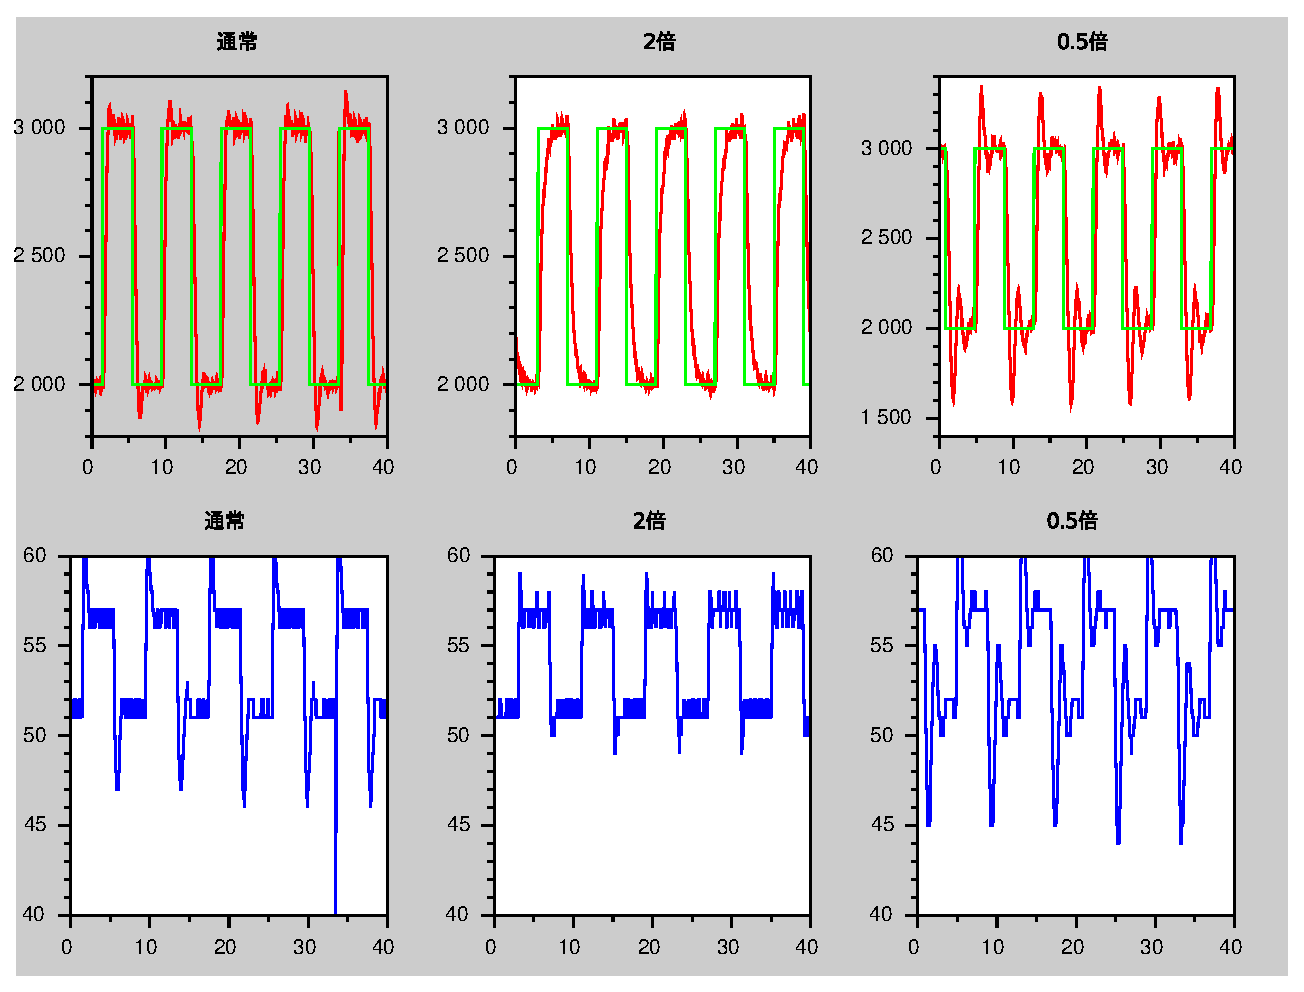
\includegraphics[width=7.0cm]{images/kadai6-1-3.eps}
\caption{課題6.1-3のグラフ}
\label{fig:kadai6-1-3}
\end{center}
\end{figure}

グラフから,$K_P$の値を大きくすると,反応速度が早いかわりに不安定になるはず!

なんかグラフおかしいっぽい????要チェック


\subsection{$K_I$の影響}
課題6.1-4の結果を報告せよ.$K_I$の値の違いによる応答の違いをグラフを用いて説明せよ.$K_I$の役割や調整の仕方について考察せよ.Scilabによるグラフの作成では,3つの応答の時間軸を調整して1つのグラフに描き,時定数などを比較できるようにせよ.

以下図\ref{fig:kadai6-1-4}に,$K_P$の値を変えず$K_I$の値を1倍,2倍,0.5倍としたときのグラフを示す.

\begin{figure}[H]
\begin{center}
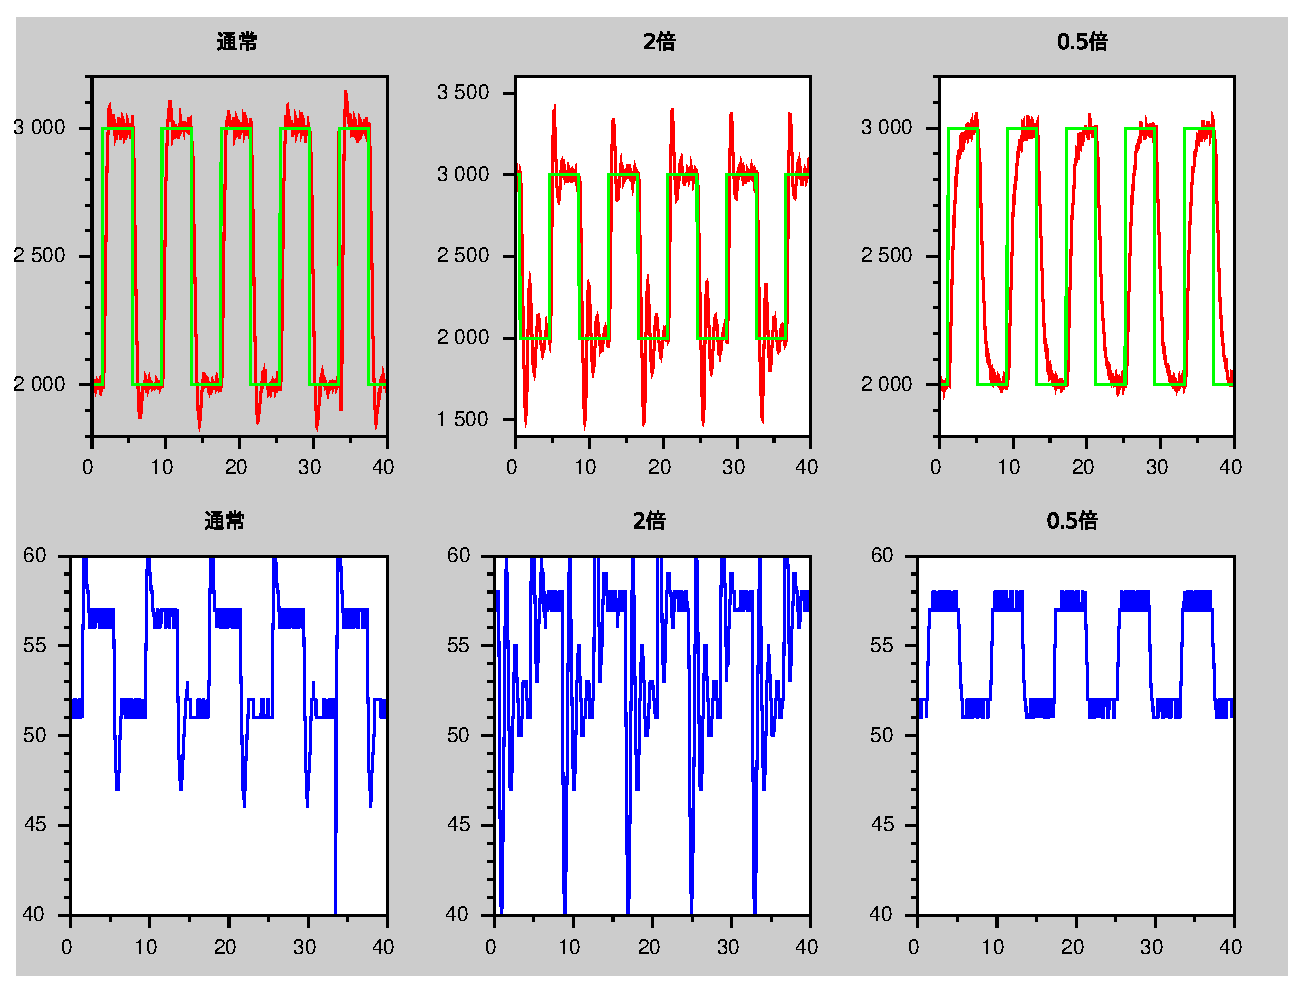
\includegraphics[width=7.0cm]{images/kadai6-1-4.eps}
\caption{課題6.1-4のグラフ}
\label{fig:kadai6-1-4}
\end{center}
\end{figure}

グラフから,$K_I$の値を大きくすると時定数が小さくなり応答速度は早くなるが,目標の出力を大きく超えたり,大きく下回ったりと不安定な出力が得られた.また$K_I$の値を小さくすると時定数が大きくなり応答速度は遅くなるが,比較的安定した出力が得られた. \\
P制御では誤差信号を$e(t)$,比例フィードバックゲインを$K_P$としたときの出力は
\begin{equation}
u(t) = K_P \times e(t)
\end{equation}
となるが,PI制御では積分ゲインを$K_I$としたとき,出力は
\begin{equation}
u(t) = K_P \times e(t) + K_I \times \int_0^t e(t) dt
\end{equation}
となり,目標値と出力の差に比例する項に加えて,目標値と出力の差の積分値に比例する項が追加される.$K_I$の役割は誤差の積分値への重み付けであるが,$K_I$の値を大きくすると,2次遅れ要素以上のシステムでは振動してしまうため,システムによってゲインを大きくするべきかそうでないかを検討する必要がある.

\section{ストロボフラッシュ}
\subsection{目的}
課題6.2の目的は何か?50字以上で答えよ. \\

課題6.2では,モータの回転速度をストロボフラッシュの原理を用いて可視化した.白黒パターンを用いることで,グラフ化をせずともすぐに目標回転速度と合っているかどうか確認するシステムの構築を確認した.

\subsection{実験結果}
課題6.2の結果を報告せよ.その際,モータの回転速度,duty比,目標回転速度などのデータをScilabを用いてグラフにすること.回転盤がどのような状況の時にどのように見えたか説明せよ.

以下図\ref{fig:kadai6-2}に課題6.2の結果を示す.

ここを追加する!!!!
\begin{figure}[H]
\begin{center}
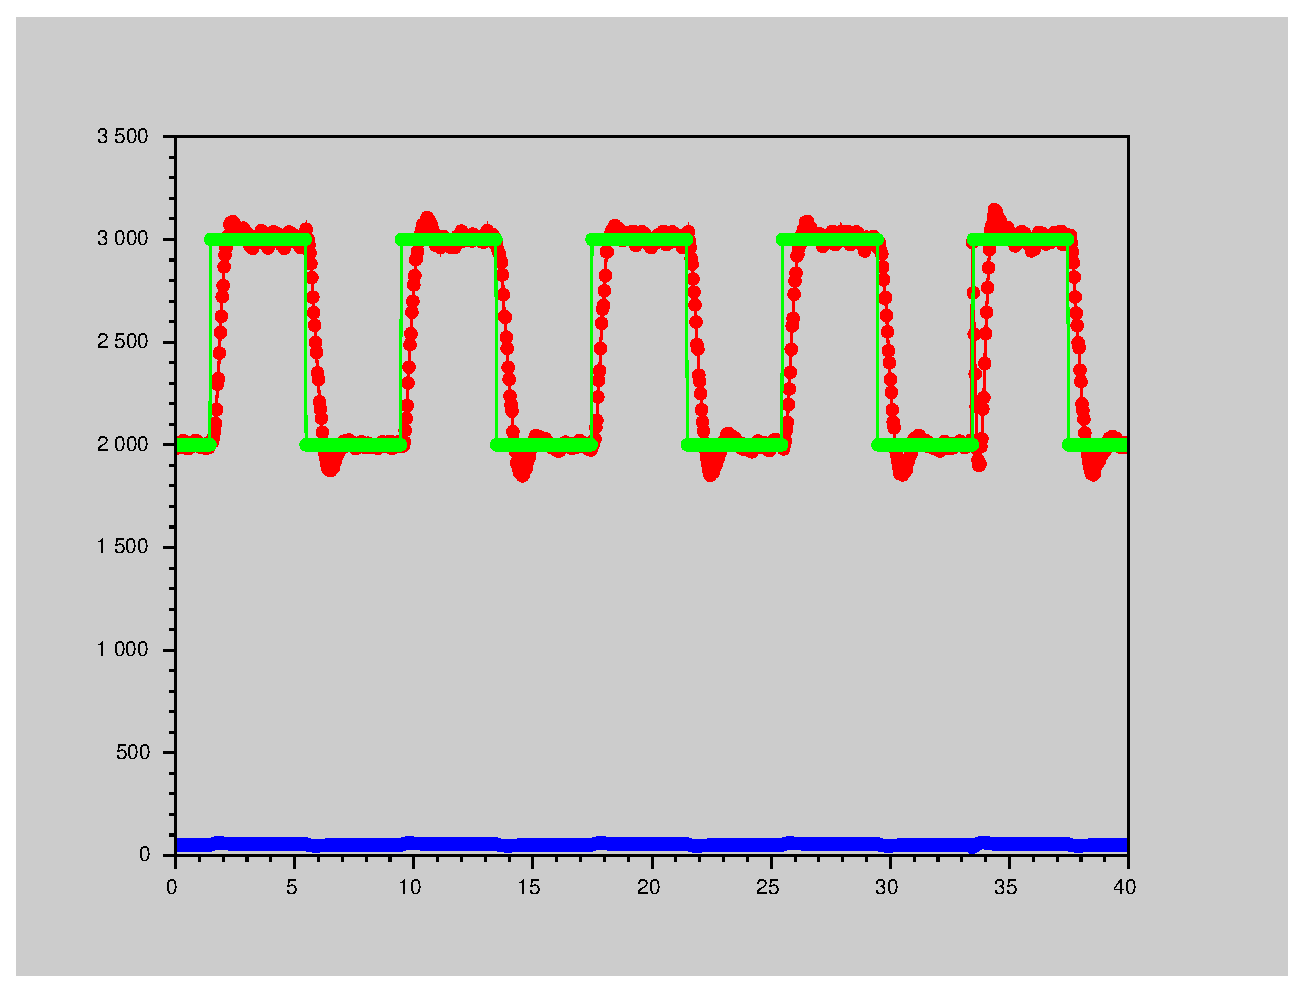
\includegraphics[width=7.0cm]{images/kadai6-2.eps}
\caption{課題6.2のグラフ}
\label{fig:kadai6-2}
\end{center}
\end{figure}

\section{原点移動の影響}
\subsection{目的}
発展課題6.1の目的は何か?60字以上で答えよ.\\

フィードバック制御における$u(t),y(t)$は動作点からの偏差である.非線形システムを線形近似する場合,動作点近傍における線型近似モデルにもとづいて制御が可能だが,原点移動をせずに動作点近傍でない場所でフィードバック制御を行った場合どうなるかを確認し,フィードバック制御における原点移動の重要性を理解することを目的とした.

\subsection{実験結果}
発展課題6.1の結果を報告せよ.その際,Scilabを用いて,モータの回転速度,duty比,目標回転速度などのデータを比較が容易になるように工夫してグラフにすること.また,$(U_0,Y_0)$の値の違いにより,応答にどのような違いが表れたか説明せよ.また,その違いの原因について考察せよ.

以下
\end{document}
